In this work we introduce the software API and tools of the \textbf{OpenSoT} framework. Moreover we show a large set of examples of high-level tasks as well as tests to evaluate the \textbf{OpenSoT}'s tasks and constraints. 
This set of tests and examples demonstrate the performances of the library and the easiness of writing complex sets of tasks and constraints.
This paper is a complement to the first part where the theoretical foundation of the frameworks were presented. 

\section{Development Pipeline}
Part of the work in developing the hardware and software for the DRC competition entry of the WALKMAN robot involved organizing the efforts of a big team that needed to work under high pressure and deliver results in a very short amount of time. During one year and a half, a whole robot was built from scratch, together with a whole simulation framework, low level joint control, middleware for interfacing the low level with the high level control, high level component model and UI for teleoperation.
Part of the work needed to feature such an achievement has involved adopting a build system.
The \emph{YCM} framework developed by the iCub facility department in Istituto Italian di Tecnologia has been used for the WALKMAN project, and an optimal development flow has been designed for the large team. 
The second fundamental aspect has been that of adopting a continuous build system and writing a very large set of unit and integration tests, especially for the core libraries and the high level control libraries.
The GIT distributed source code managament system has been used, with gitlab used for hosting an environment for collaboration, issue-tracking and documentation sharing via its WIKI system.

\section{Component Model}
The compoment model developed is based on the yarp framework and named GYM.
It contains a logging and configuration mechanism, paramHelper, for which a UI has been developed for online gain tuning. GYM provides facilities for automatic module creation. Every module is composed of a low frequency thread that accepts high level management commands, and a high frequency thread that takes care of the control and obtains sensor feedback from the robot and task level commands by the user.

\section{Simulating and Controlling Compliant Robots}
The simulator is a fundamental part of the framework and the robot software development cycle as the first step to validate algorithms, thus minimizing the risks of hardware failures.
In these frameworks, the \emph{simulator} is a module that represents the real robot at the interface level (Figure \ref{yarp_simulation}). Such simulator module accepts control input (desired joint torques, desired joint position, ...) and outputs sensory feedback (cameras, joint positions, ...) from the simulated world. These simulators usually allow to have the human in-the-loop permitting to train a human operator. The most important aspect is that they allow to develop modules that directly will work in the real robot without any need to rewrite code. In fact, when the real robot is used, there is a module that replaces the simulator by providing the same hardware interfaces. 

\begin{figure}[h!]
  \centering
    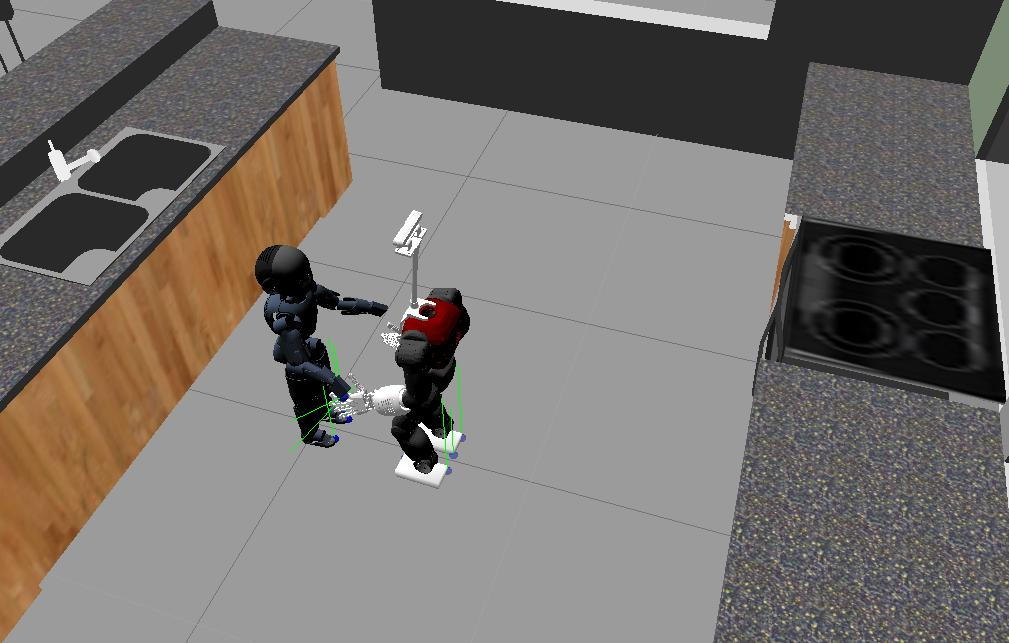
\includegraphics[width=0.475\textwidth]{images/coman_icub_gazebo.jpg}
    \caption{COMAN and iCub interacting inside a Gazebo simulation of a kitchen. Blue dots represent contact points.}\label{coman_icub_gazebo}
\end{figure}

With these concepts in mind we decided to extend one of the most known robotics simulator, Gazebo (\cite{koenig2004design}), to be compatible with one of the most used robotics framework, YARP (Figure \ref{coman_icub_gazebo}), developed in the Italian Institute of Technology. 
YARP is supported by the iCub simulator (iCubSim, \cite{Tikhanoff:2008:OSC:1774674.1774684}) that is dedicated to a specific platform. The needs of a more generic tool for simulating different robots rise up. 
Gazebo, which has been recently chosen as the simulator for the DARPA Virtual Robotic Challenge (VRC, \cite{DRC}), allows the use of different dynamic engines, it is easily expandable through plugins and it has a strong and active community. Gazebo is maintained by the Open Source Robotics Foundation (\cite{OSRF}).

\label{structure}
It is useful to understand Gazebo plugins and YARP device drivers before describing the structure of our plugins (from now on \emph{gazebo\_yarp\_plugins}).

Gazebo plugins are C++ classes that extend the functionalities of Gazebo, while YARP device drivers are C++ classes used in YARP for abstracting the functionality of robot devices.
Usually, each class of gazebo\_yarp\_plugins embeds a YARP device driver in a Gazebo plugin. 

{\bf Gazebo Plugins}
A plugin is a piece of code compiled as a shared library and inserted into the simulator. A plugin has direct access to all the functionalities of Gazebo from the physics engine to the simulated world. Furthermore, plugins are self-contained routines that are easily shared and can be inserted and removed from a running system. There are 4 types of plugins in Gazebo: \textbf{world}, \textbf{model} and \textbf{sensor} plugins are attached to and control a specific simulated world/model/sensor respectively, while \textbf{system} plugin is specified on the command line and loads during the Gazebo startup.


{\bf YARP \emph{Device Drivers}}
YARP provides special devices that act as network proxies and make interfaces available through a network connection. This allows accessing devices remotely across the network without code change.

A device driver is a class that implements one or more interfaces. There are three separate concerns related to devices in YARP:
\begin{itemize}
\item Implementing specific drivers for particular devices
\item Defining interfaces for device families
\item Implementing network wrappers for interfaces
\end{itemize}
For example the Control Board device driver implements a set of interfaces that are used to control the robot (IPositionControl, ITorqueControl, etc.) and another set of interfaces to read data from the motors (IEncoders, etc).

\subsection{Gazebo-YARP Plugins}
The gazebo\_yarp\_plugins is made of:
\begin{itemize}
    \item Gazebo plugins that instantiate YARP device drivers,
    \item YARP device drivers that wrap Gazebo functionalities inside the YARP device interfaces.
\end{itemize}
The plugins/devices already implemented are the \emph{Control Board}, \emph{6-axis Force Torque sensor}, \emph{Inertial Measurement Unit} (IMU) and a \emph{Clock} plugin used for synchronization.
The first three plugins are directly related to the simulated objects and sensors, while the last one is a system plugin that synchronizes all the other YARP modules with the simulation time. 

\begin{figure}
        \centering
        \begin{subfigure}[b]{0.475\textwidth}
                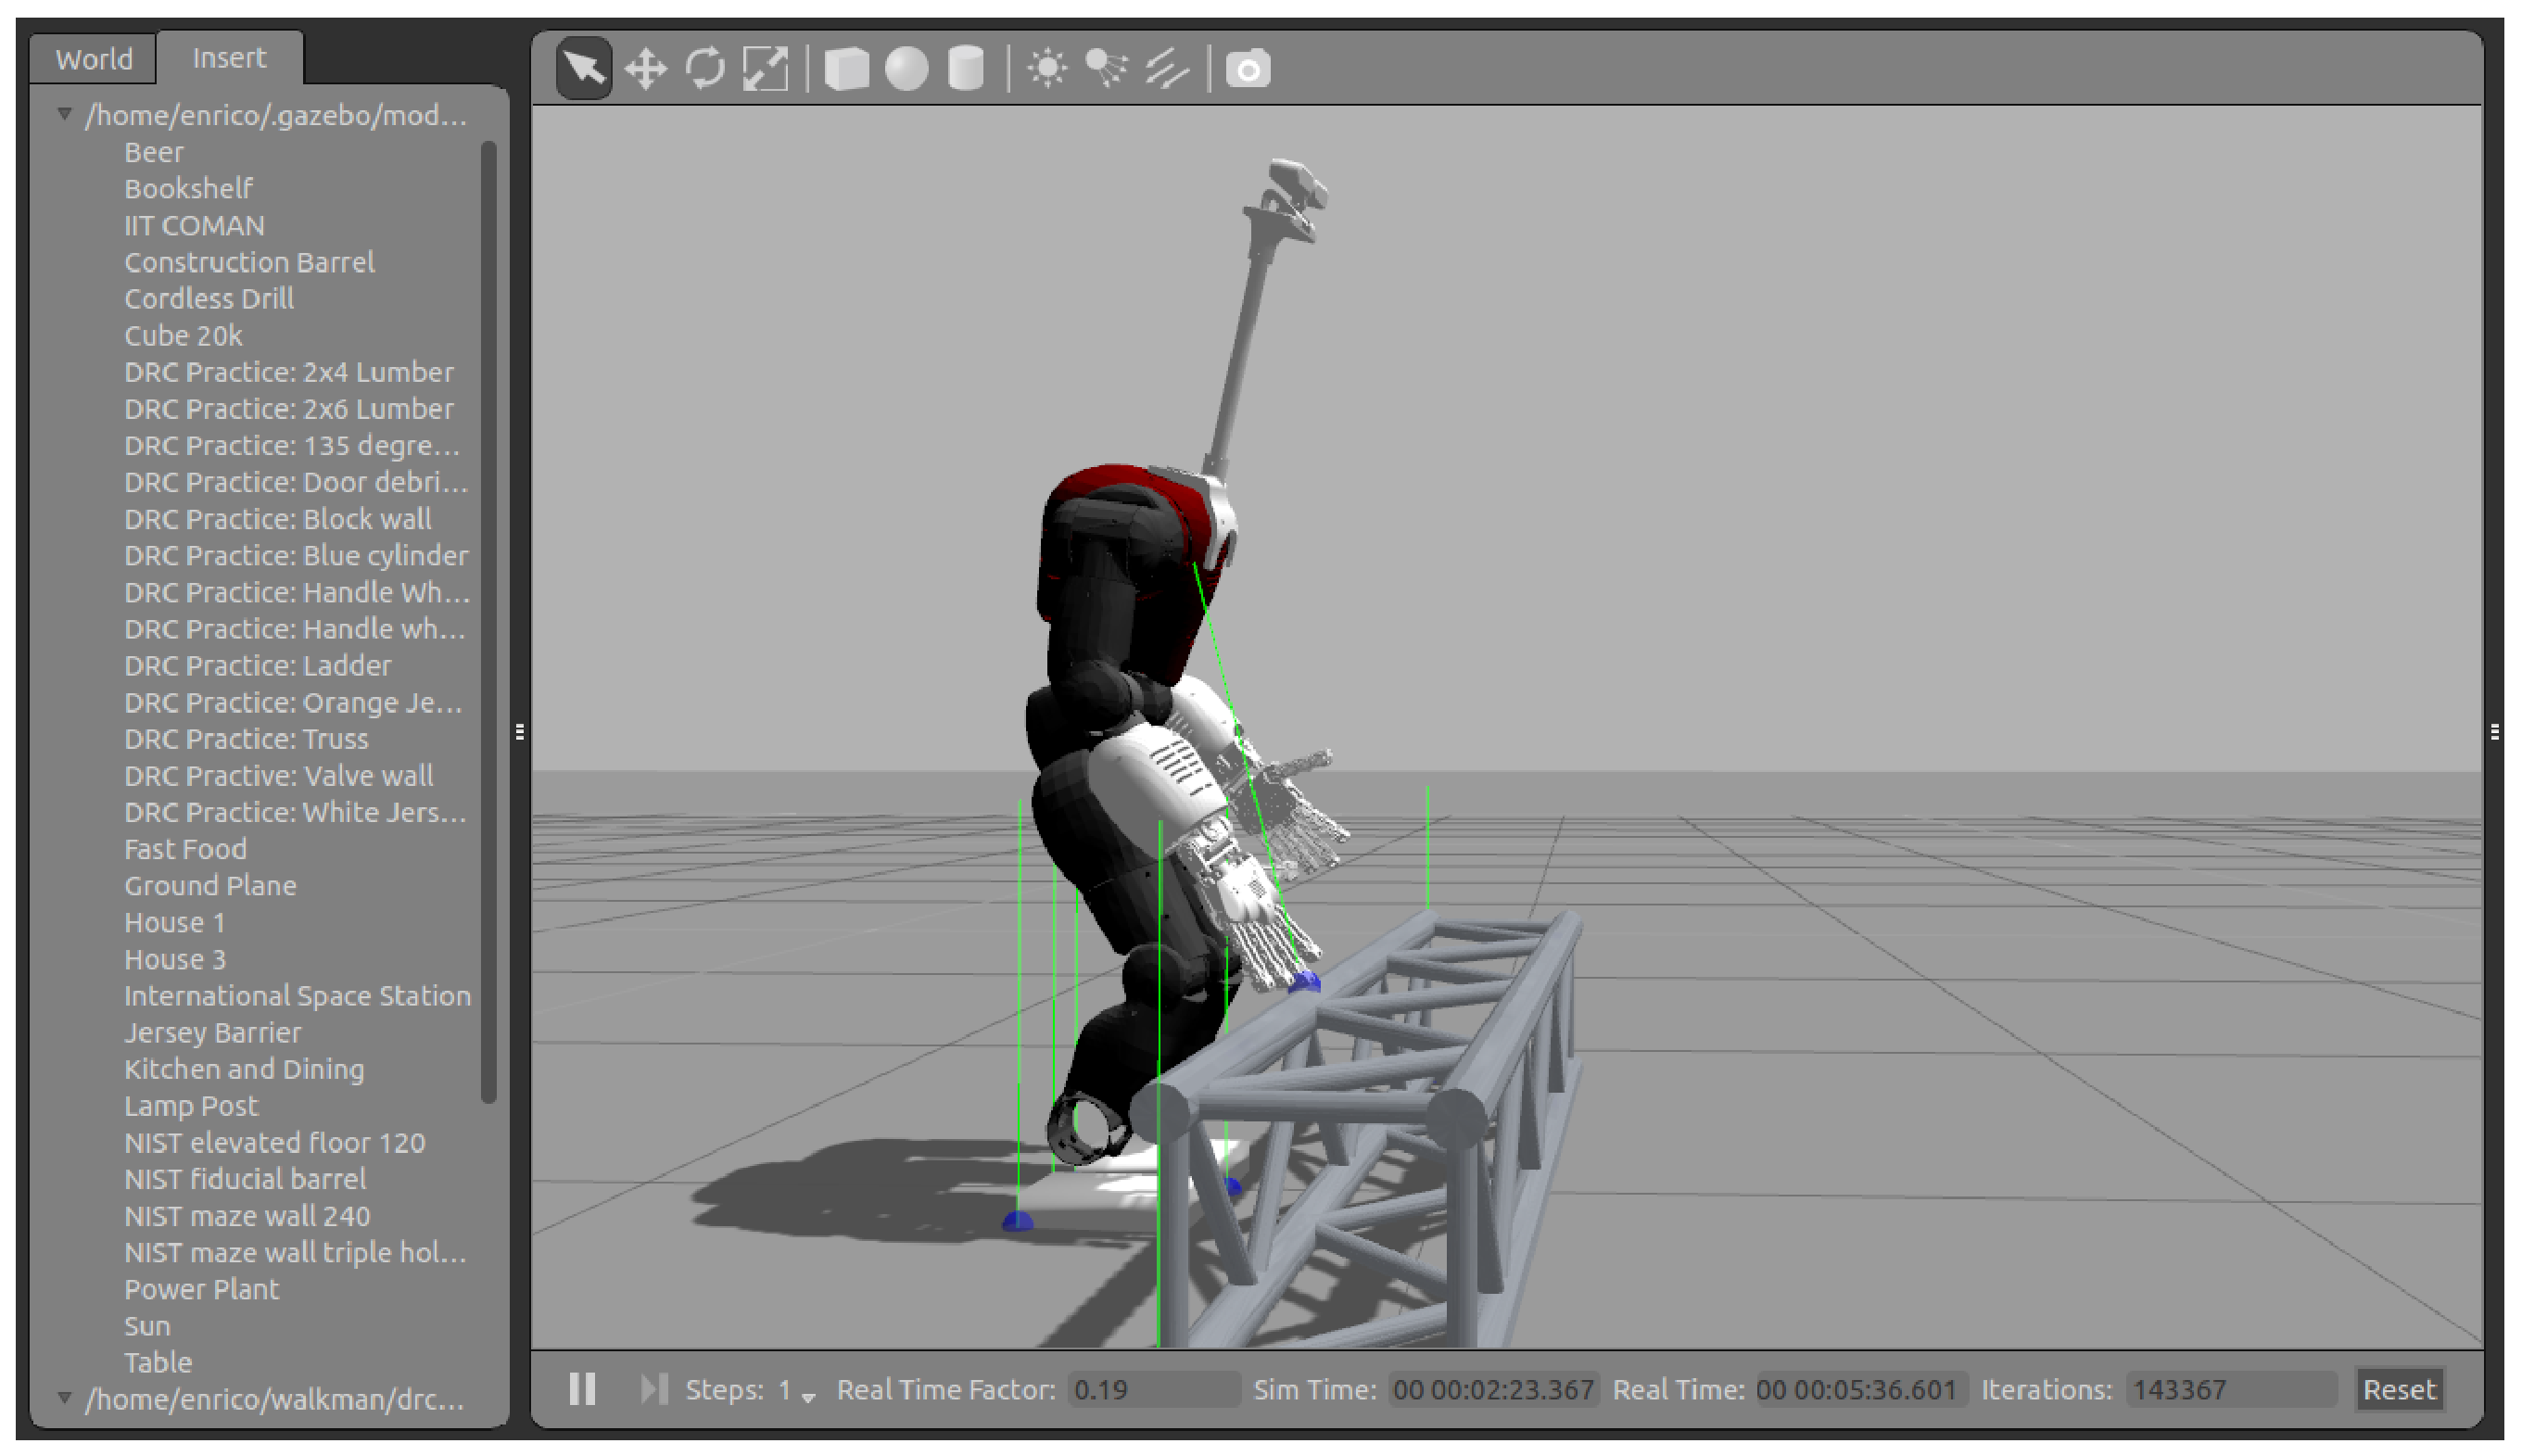
\includegraphics[width=\textwidth]{images/coman_ft_a.eps}
                \caption{Gazebo interface with COMAN}
                \label{yarp_simulation_coman_a}
        \end{subfigure}%
        \\
        \begin{subfigure}[b]{0.475\textwidth}
                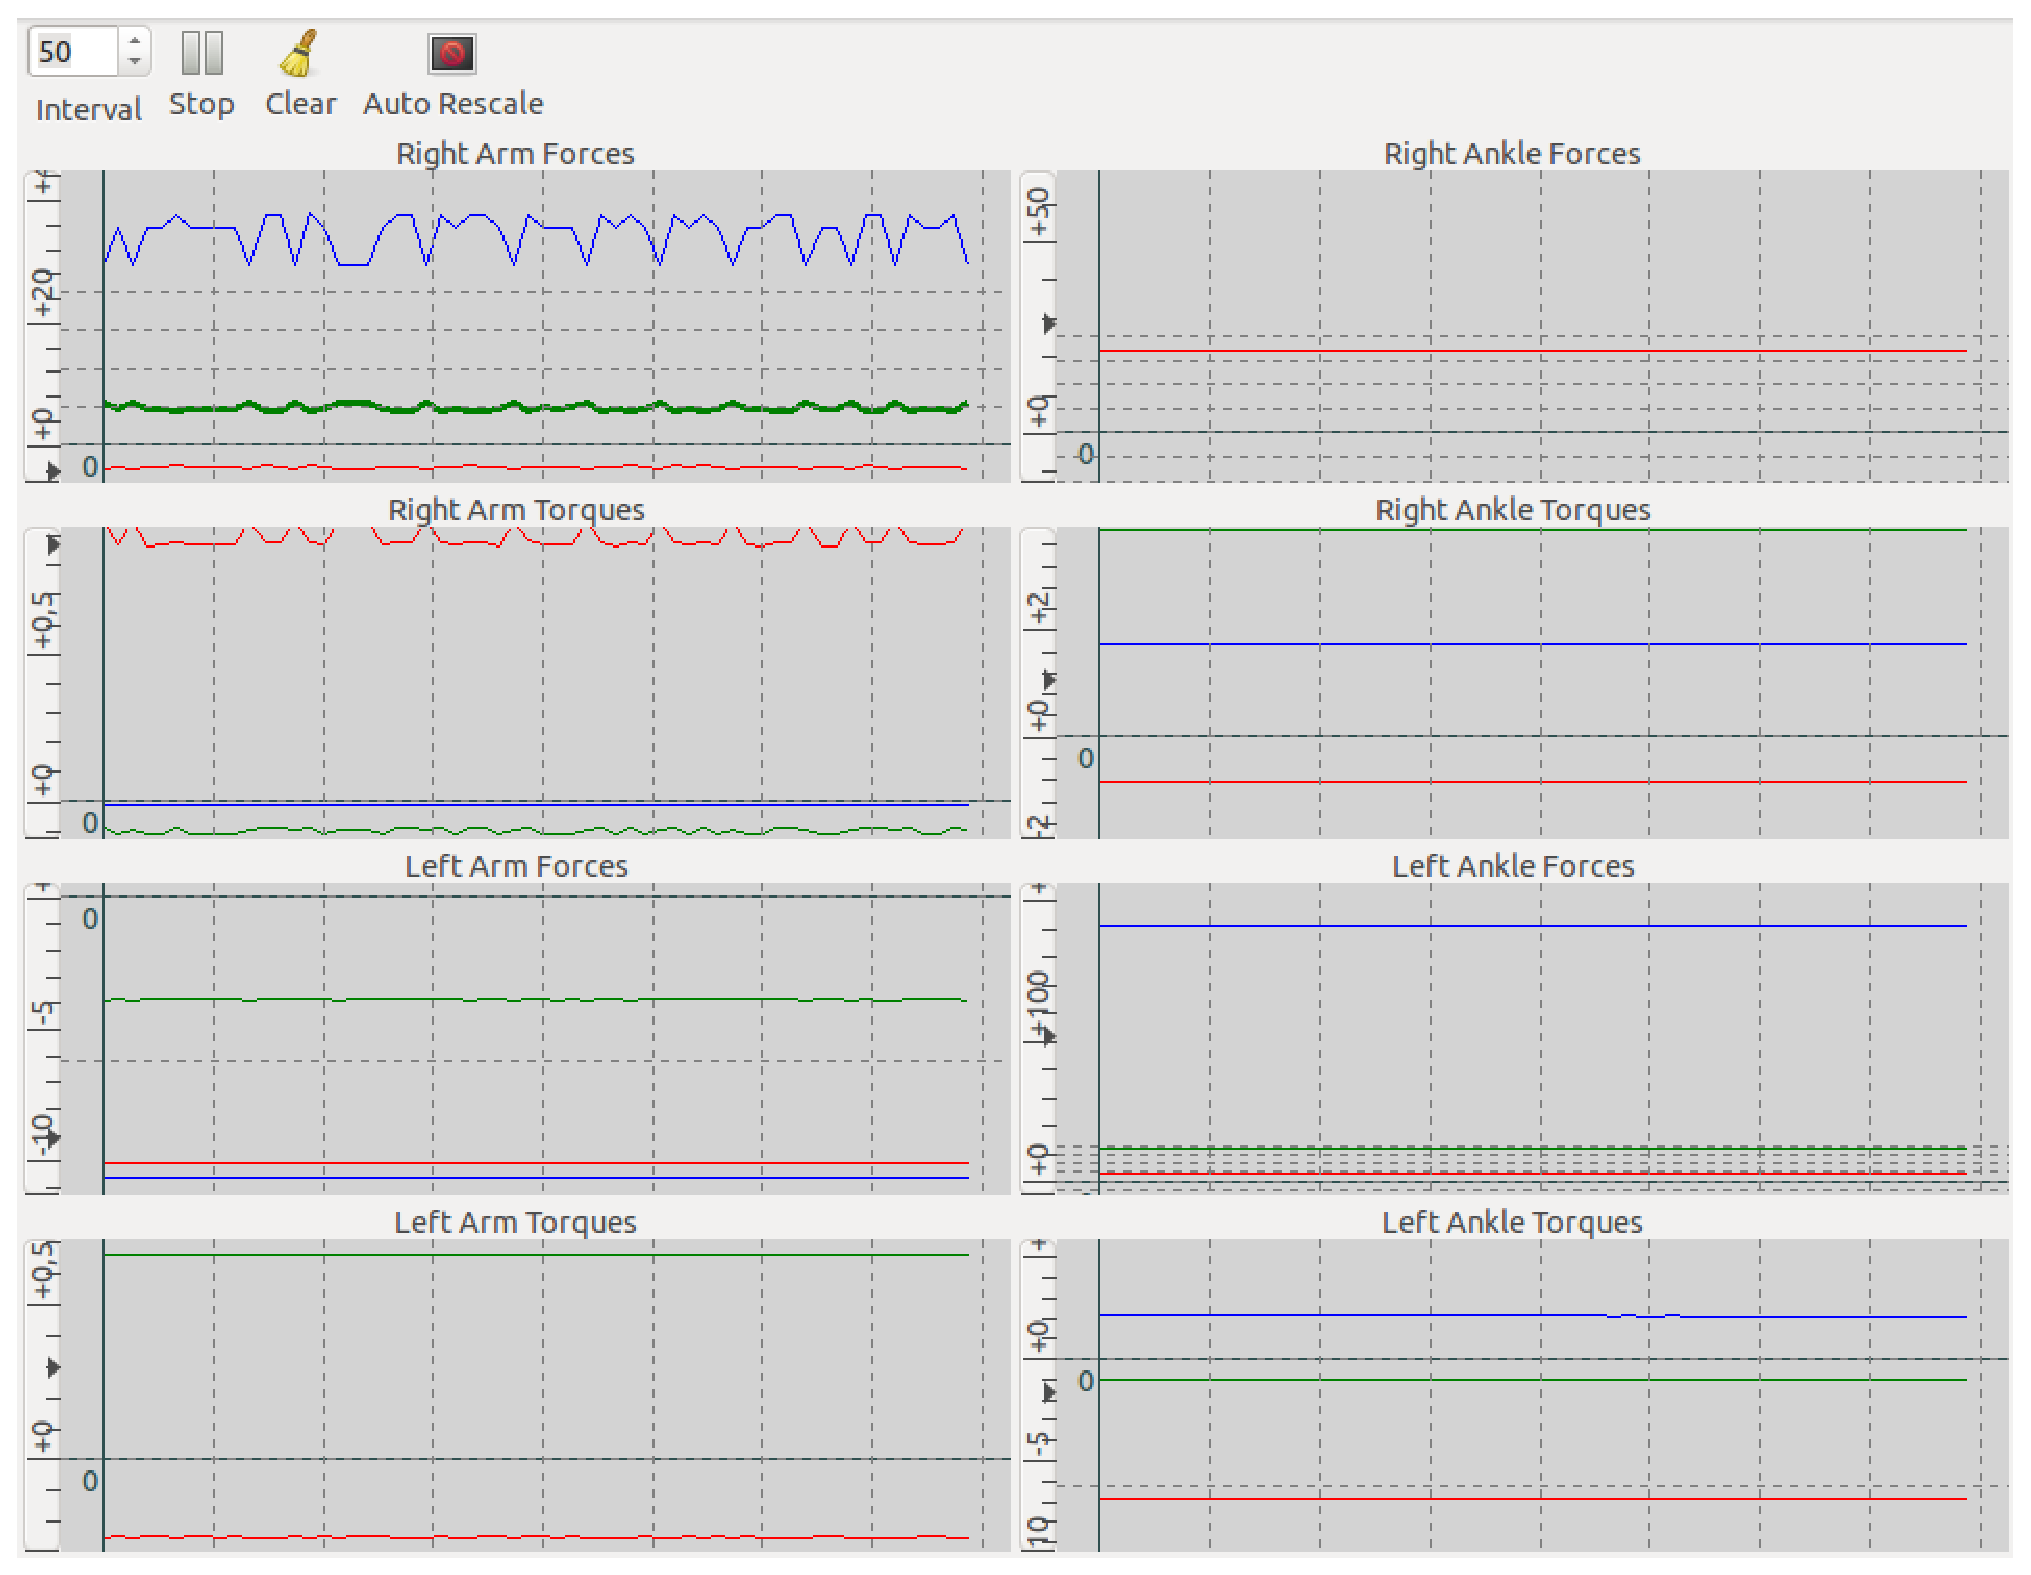
\includegraphics[width=\textwidth]{images/coman_ft_b.eps}
                \caption{A yarpscope showing on-line the forces and the torques at each Force/Torque sensor}
                \label{yarp_simulation_coman_b}
        \end{subfigure}
        \\
        \begin{subfigure}[b]{0.475\textwidth}
                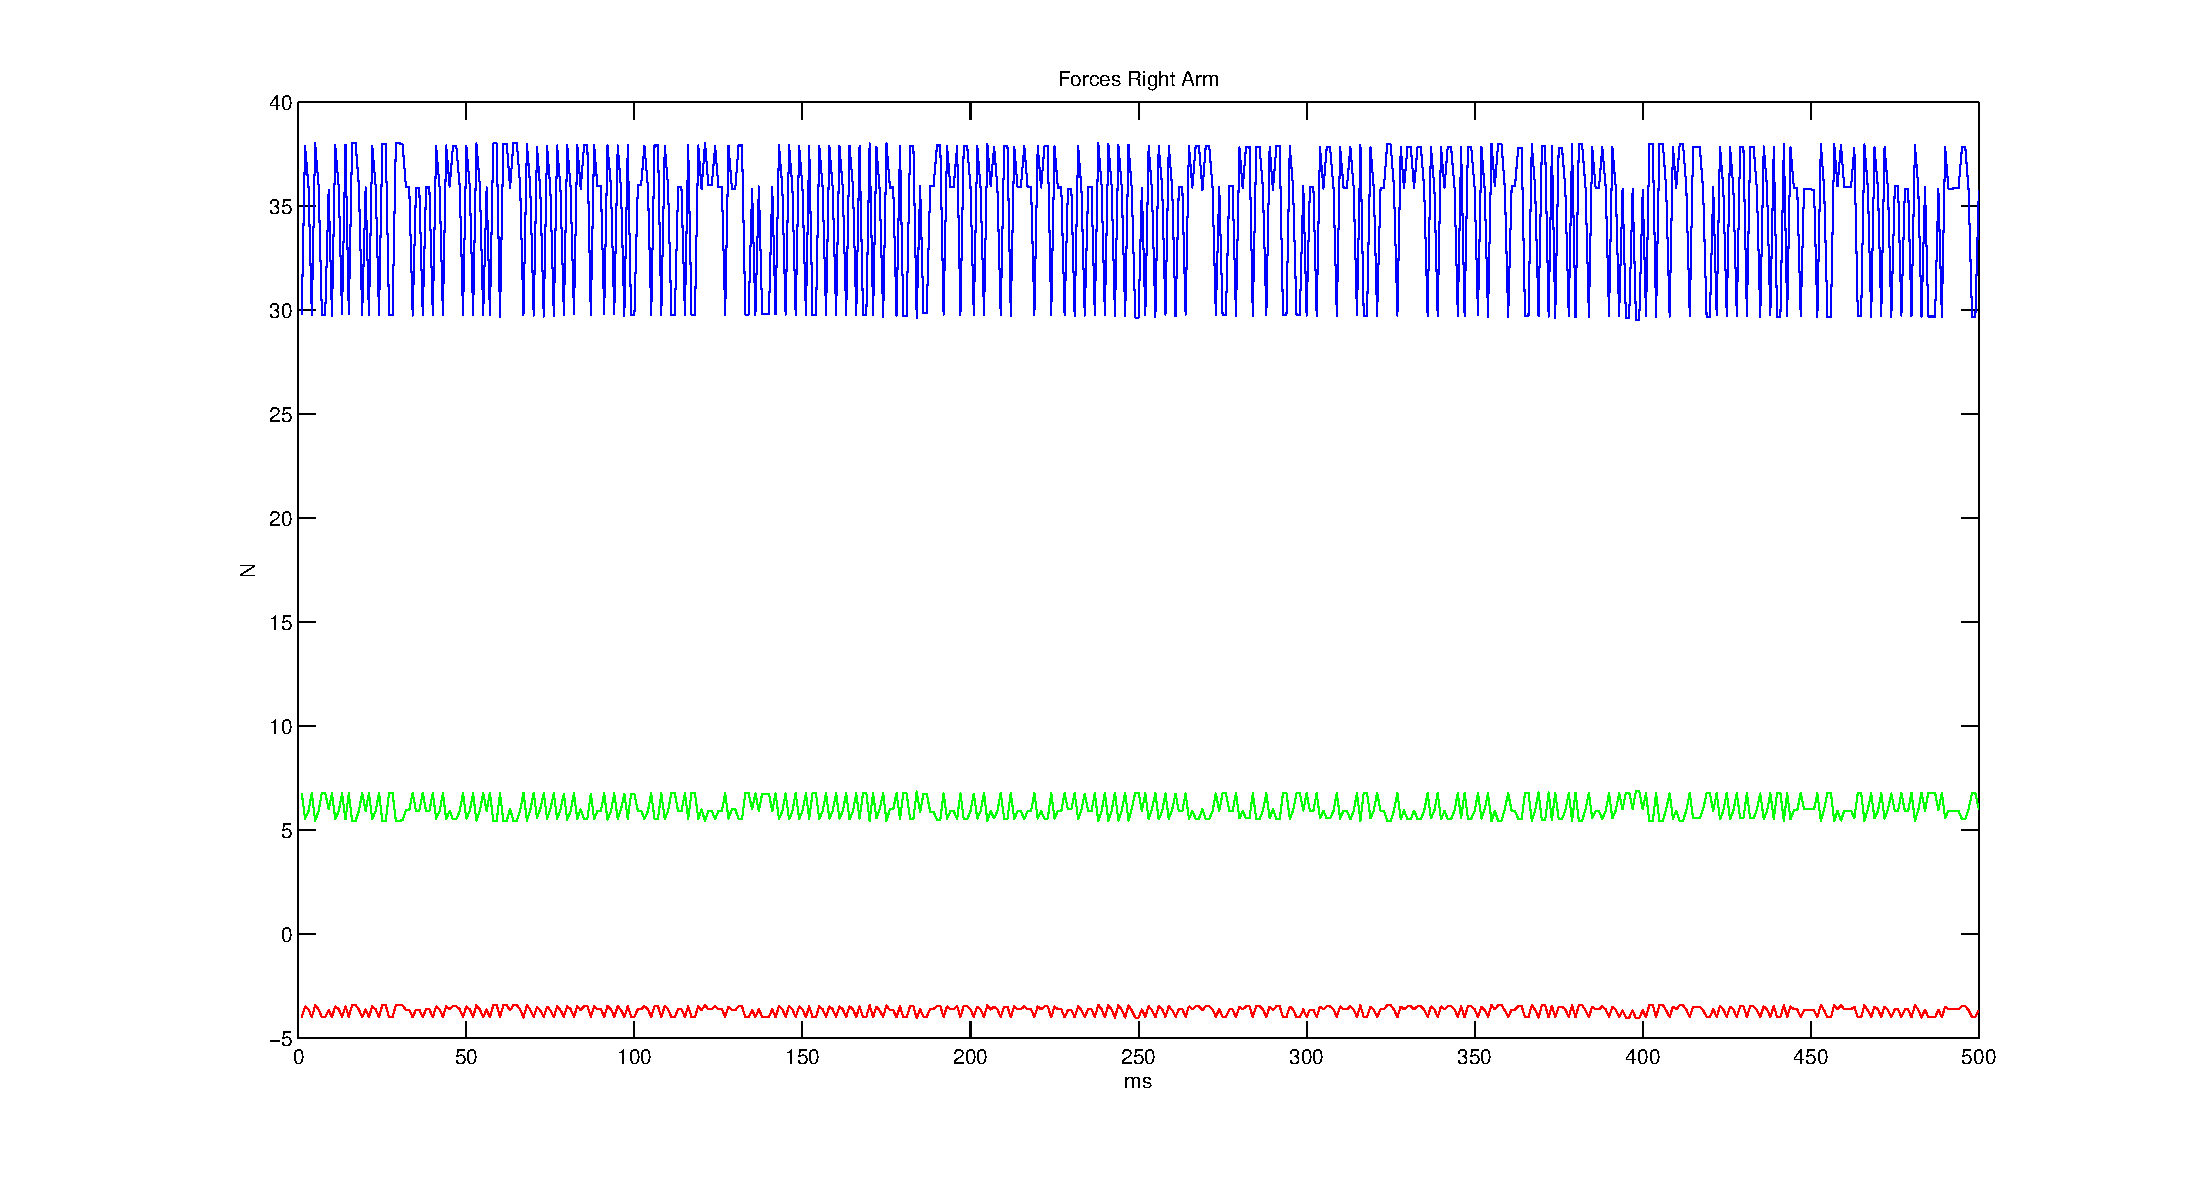
\includegraphics[width=\textwidth]{images/coman_ft_c.eps}
                \caption{Plot of forces measured at the simulated Force/Torque sensor placed on the right arm. Forces along x,y and z are respectively in red, green and blue}
                \label{yarp_simulation_coman_c}
        \end{subfigure}
        \\
        \begin{subfigure}[b]{0.475\textwidth}
                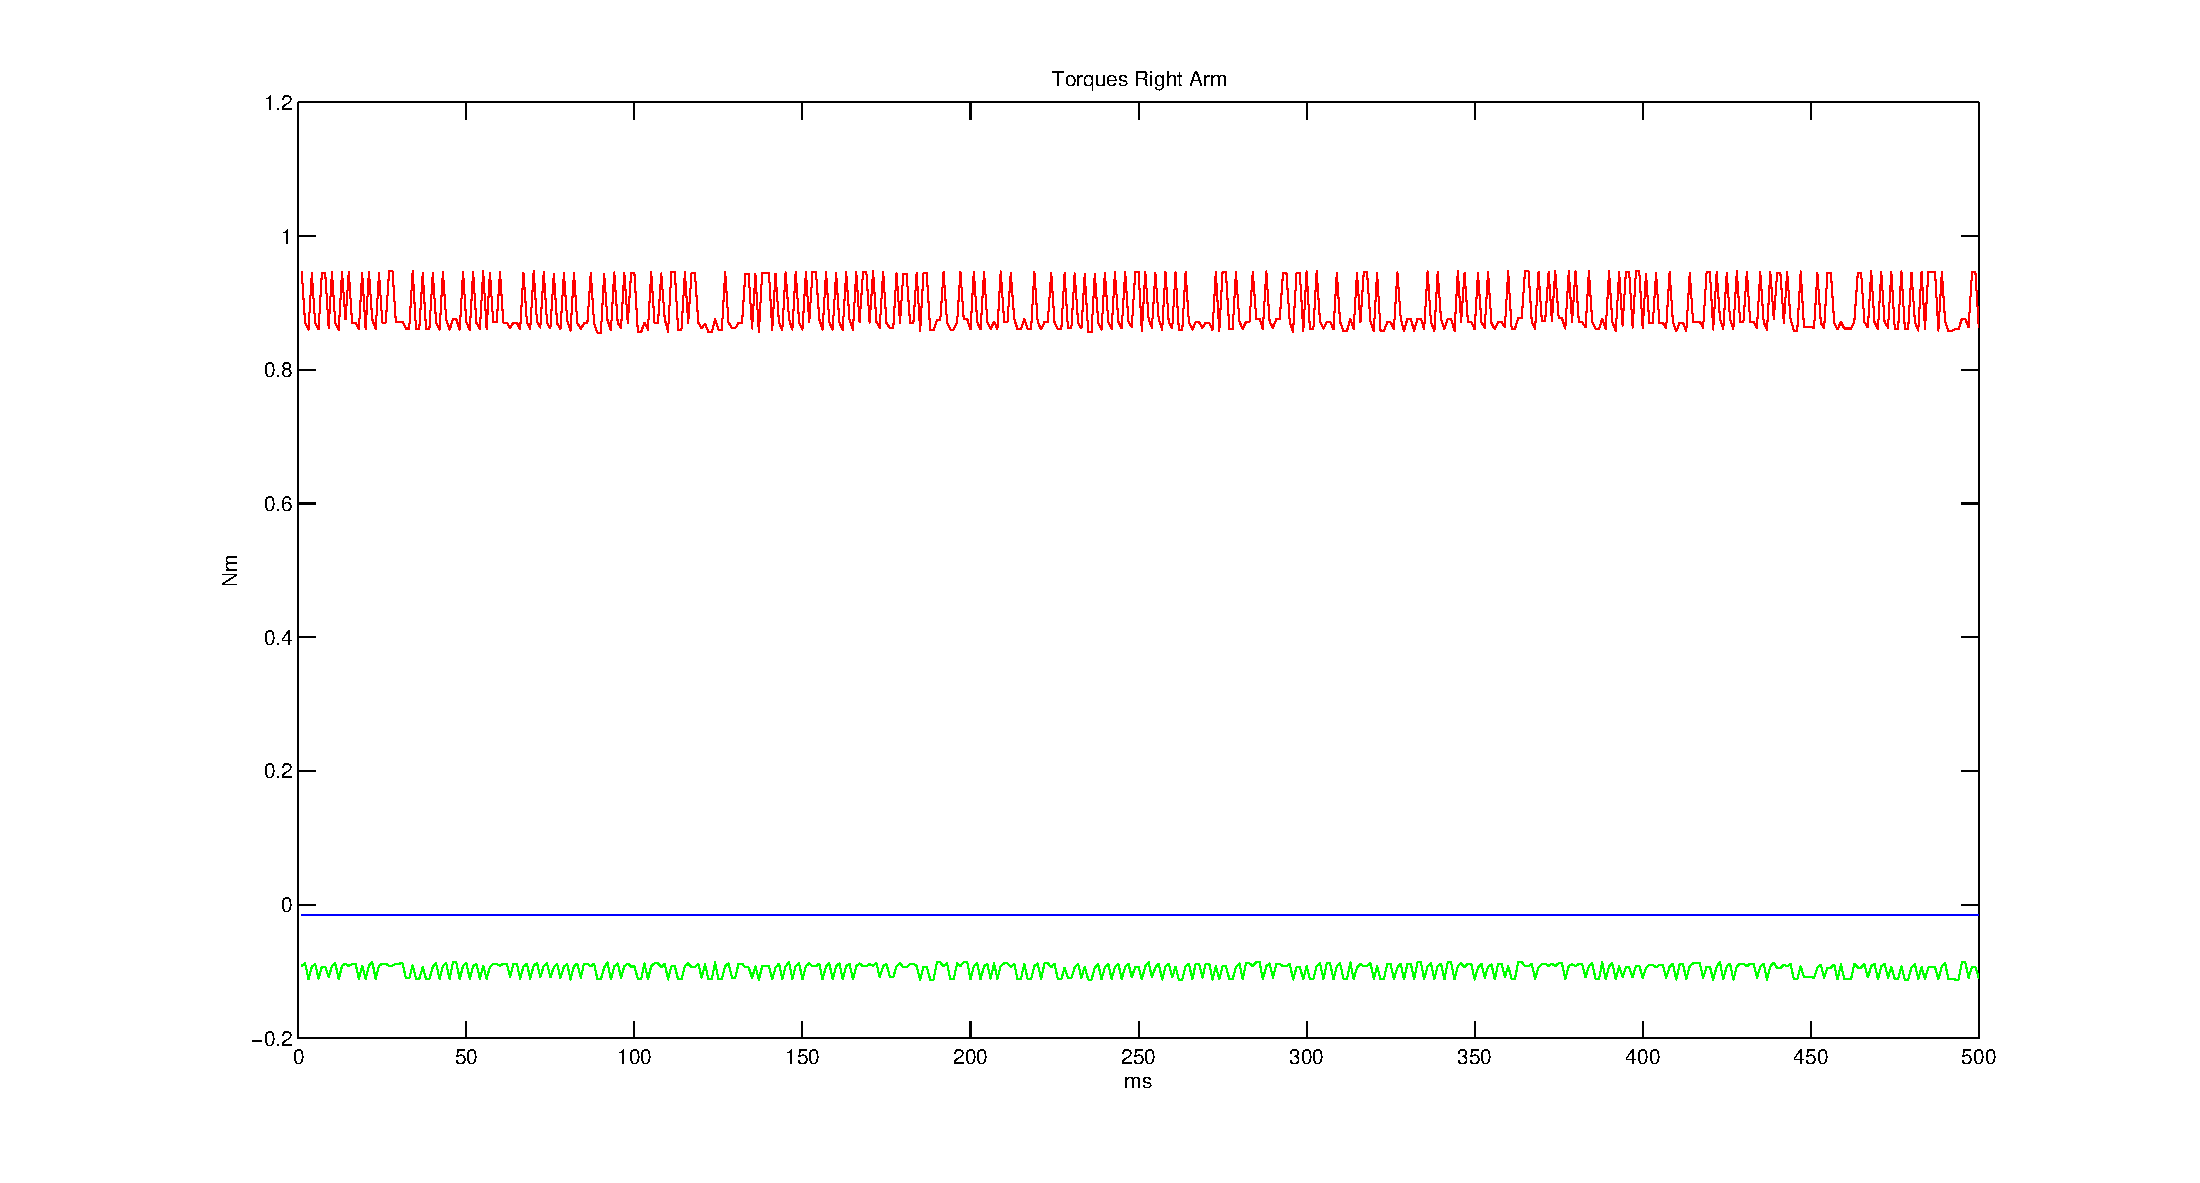
\includegraphics[width=\textwidth]{images/coman_ft_d.eps}
                \caption{Plot of torques measured at the simulated Force/Torque sensor placed on the right arm. Torques along x,y and z are respectively in red, green and blue}
                \label{yarp_simulation_coman_d}
        \end{subfigure}
        \caption{A Gazebo simulation running COMAN interacting with debris}\label{force_torque}
\end{figure}

\subsection{Control Board}
The Control Board plugin allows to control the robot using YARP Interfaces, it is implemented as a Gazebo Model plugin. Every control board allows the user to control one or more joints (a kinematic chain such as the arm or leg, etc.) as specified in a configuration file. For each controlled joint the control board opens different interfaces, permitting the use of different type of controllers for each joint. Such interfaces include position control, torque control, encoders reading, torque measurement and joint impedance control. Usually the number of instantiated control boards is equal to the number of kinematic chains. Each control board, during every cycle of simulation, reads position, velocity and torque values from the simulated joints and sends desired joints position or torques to the simulator. The values read from the simulator are broadcasted through YARP interfaces in the YARP network, in a similar way the desired joint values come from YARP interfaces (Figure \ref{control_board}). The following YARP interfaces are used to control the robot.
\begin{itemize}
\item \textbf{IPositionControl}: a position control with a linear trajectory generator considering a max joint speed
\item \textbf{IPositionDirect}: a position control using Gazebo position PIDs
\item \textbf{ITorqueControl}: a perfect torque follower
\item \textbf{IImpedanceControl}: a joint impedance control with the following law
\begin{equation}
    \tau_d = -P_d(q-q_d) - D_d\dot{q} + \tau_{offset}
\end{equation}
where $q_d$ is the desired equilibrium position, $P_d$ is the desired joint stiffness and $D_d$ is the desired joint damping. $\tau_{offset}$ is an extra signal that can be used for gravity compensation or inverse dynamics control.
\end{itemize}
Furthermore, the Control Board implements the \textbf{IControlMode} interface that allows to change the type of controller online. All these interfaces are also available on the robot and they have the same behaviour.

\begin{figure}[h!]
  \centering
    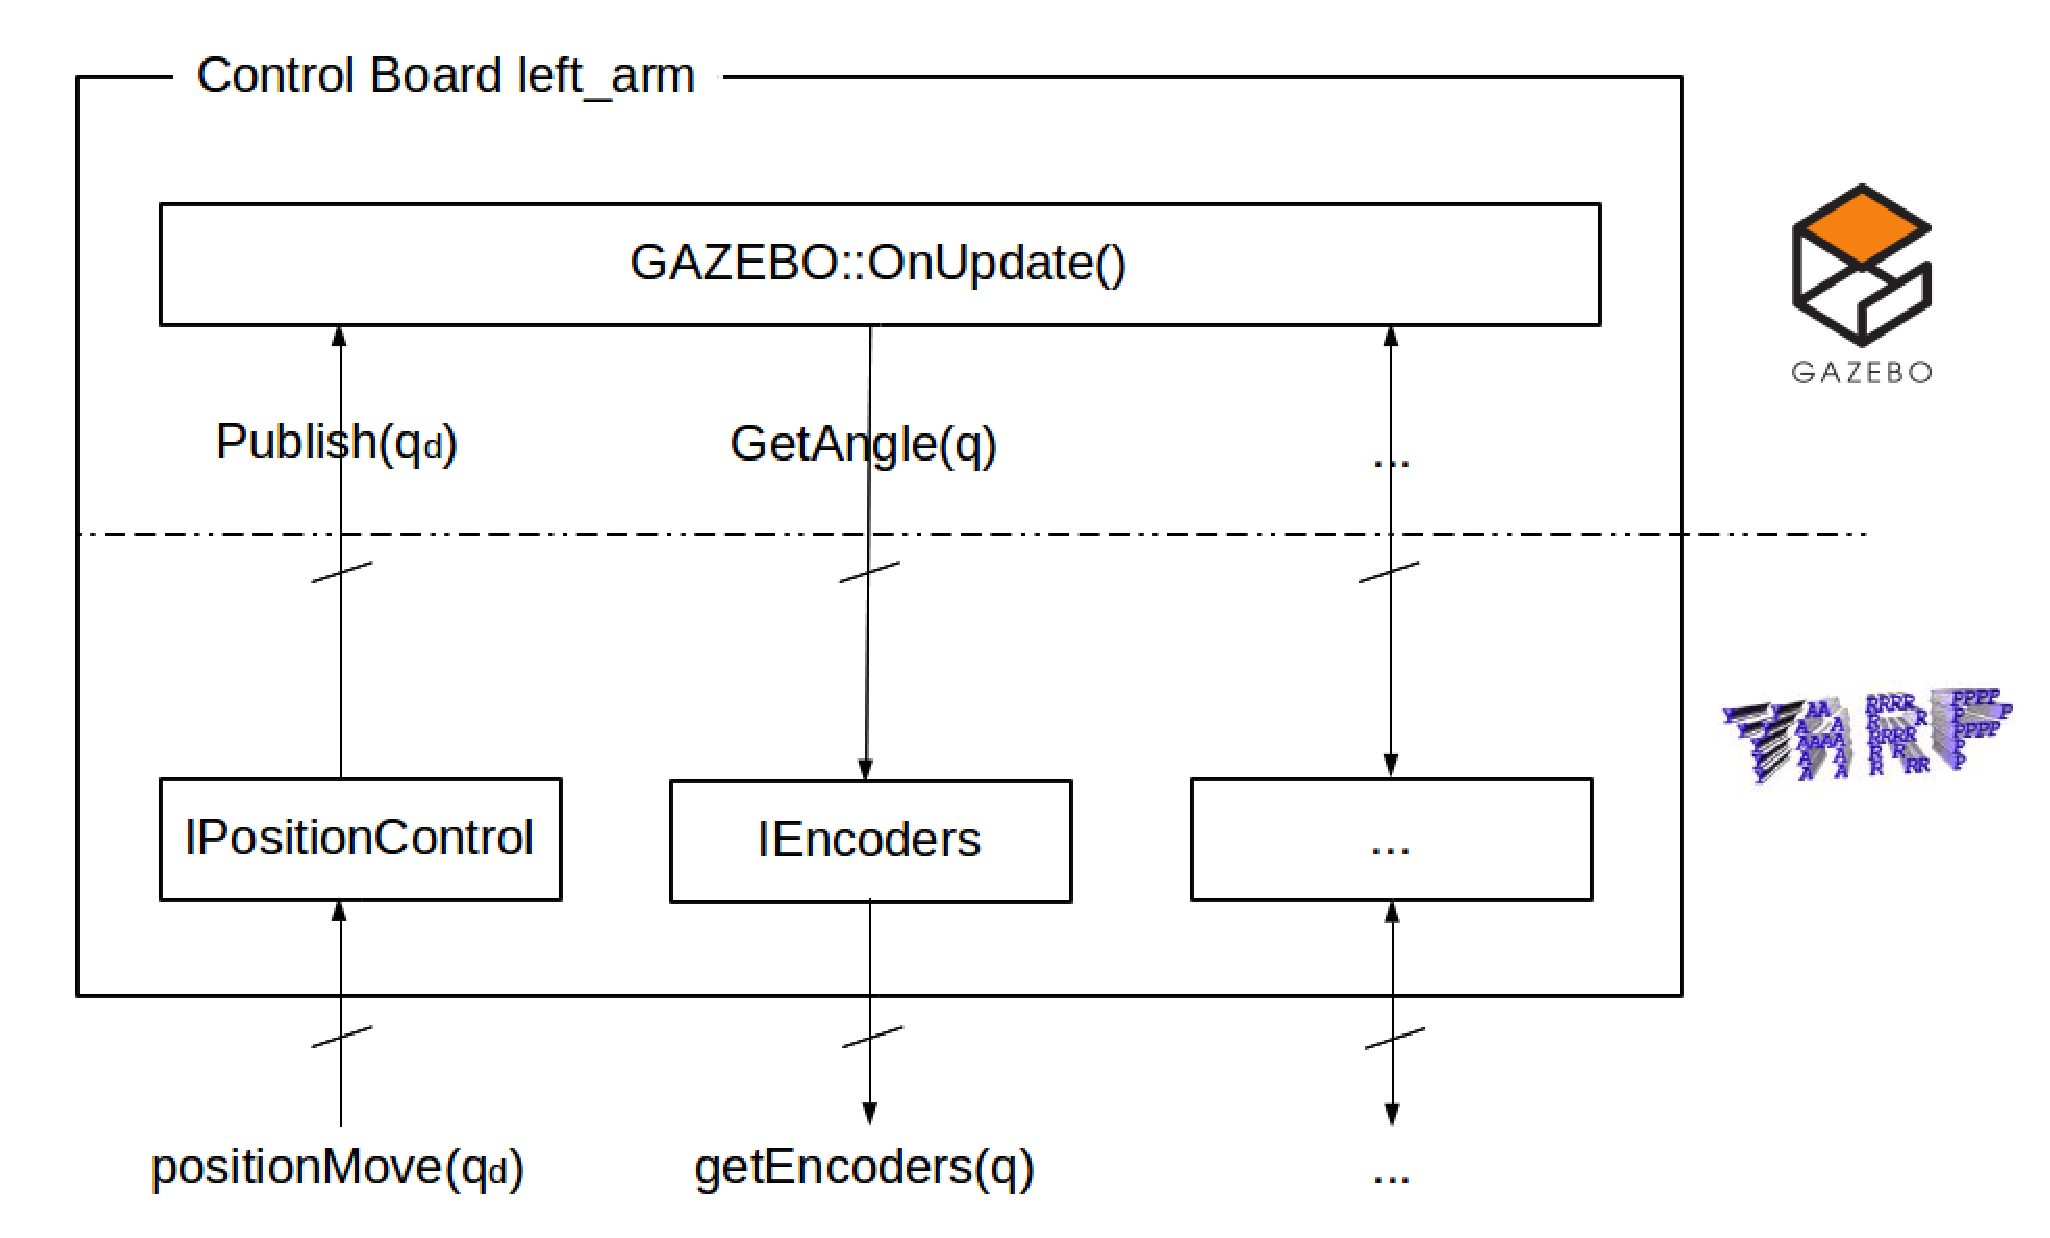
\includegraphics[width=0.5\textwidth]{images/control_board.eps}
    \caption{Control Board plugin for the left\_arm kinematic chain. yarp::IPositionControl interface has a method positionMove() that can be used to set joint values inside a YARP module. The plugin implements such interface by calling the Publish() method inside the Gazebo API to move the simulated joints at each OnUpdate().}\label{control_board}
\end{figure}

\subsection{6-axis Force/Torque sensor}
A Force/Torque sensor measures a wrench in the robot structure (Figure \ref{force_torque}). The sensor, at the time of writing, is simulated in Gazebo as if it was attached to the reference frame associated to a joint. On the YARP side, the reading of a generic sensor is implemented as a \textbf{IAnalogSensor} interface (Figure \ref{ianalog_force_torque}). The broadcasted data is a vector of six numbers representing the forces and the torques applied on that reference frame.

\subsection{IMU sensor}
An IMU measures velocity, orientation, and gravitational forces, using a combination of accelerometers and gyroscopes, of the link where it is placed. It is also possible to add white Gaussian noise on the measurement (Figure \ref{icub_inertial}).
Similar to the Force/Torque sensor, it is implemented as a \textbf{IAnalogSensor} interface.

\begin{figure}[h!]
  \centering
    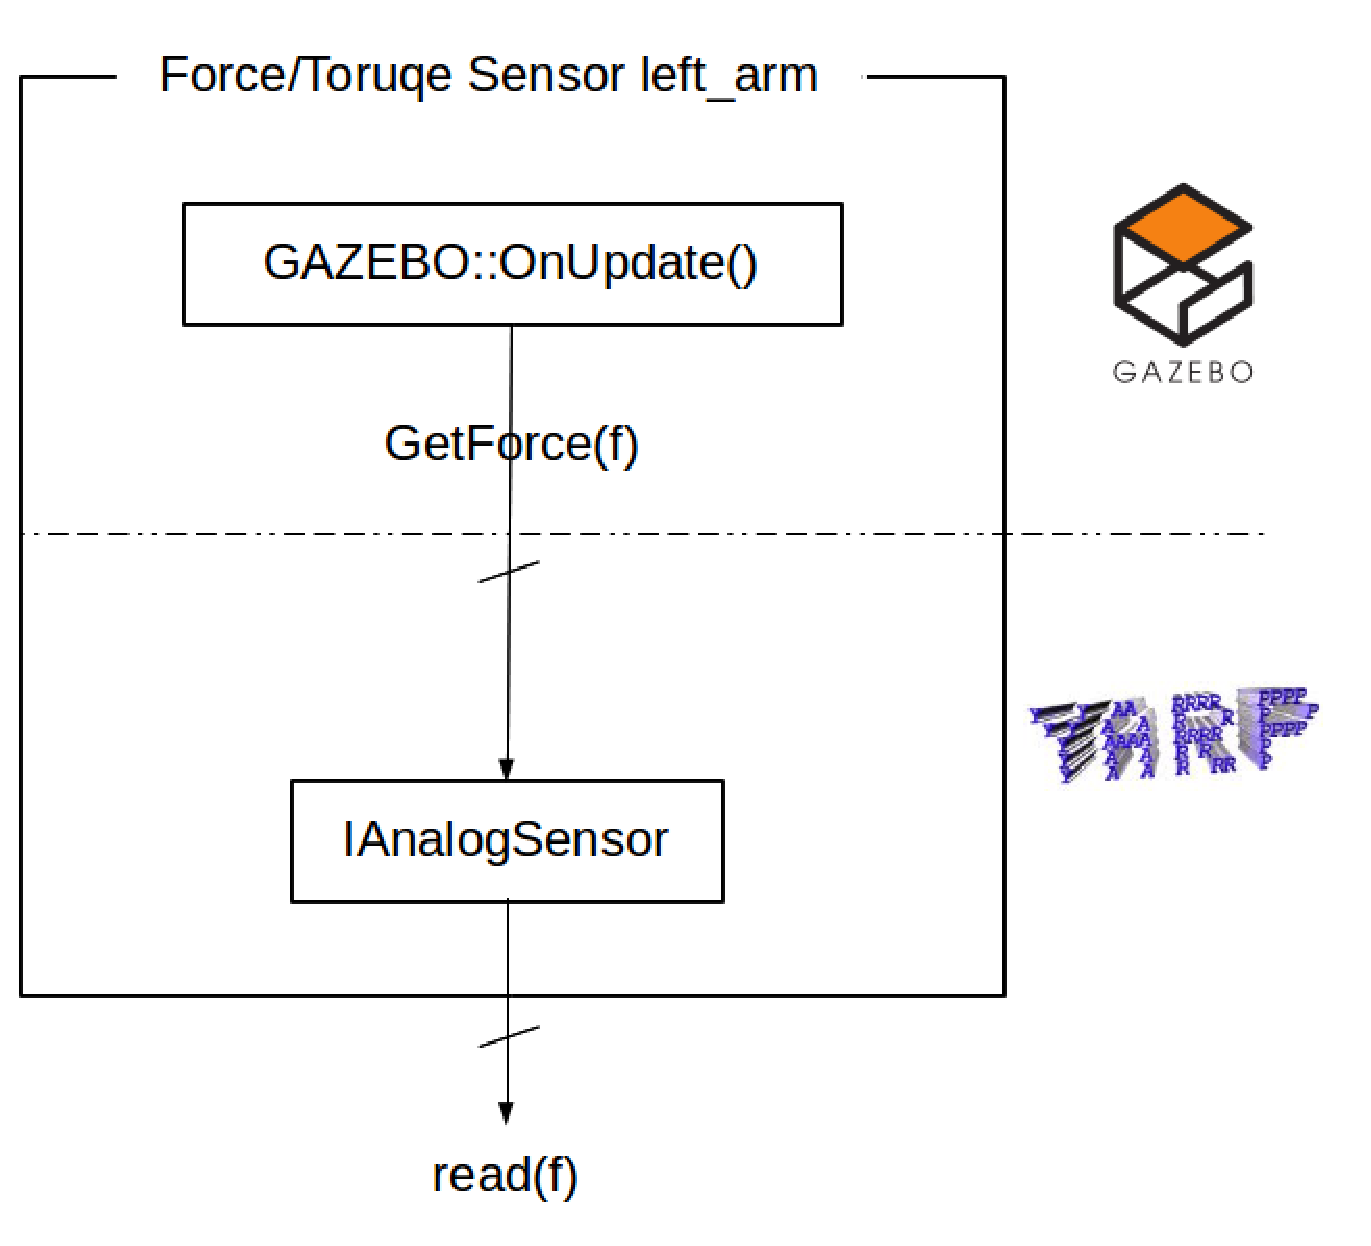
\includegraphics[width=0.475\textwidth]{images/ianalog_force_torque.eps}
    \caption{The Force/Torque sensor in the left arm is implemented as a YARP IAnalogSensor interface. At every step the internal state of the plugin is updated with the last readings of forces and torques from the simulation.}\label{ianalog_force_torque}
\end{figure}

\subsection{Simulation Description Format (SDF)}
Gazebo uses an XML-style format, Simulation Description Format (SDF), to save and load information about a simulated world or model. An SDF encapsulates all the necessary information for a simulation such as:
\begin{itemize}
\item \textbf{Scene}: ambient lighting, sky properties, shadows.
\item \textbf{Physics}: gravity, time step, physics engine.
\item \textbf{Models}: collection of links, collision objects, joints, and sensors.
\item \textbf{Lights}: point, spot, and directional light sources.
\item \textbf{Plugins}: world, model, sensor, and system plugins.
\end{itemize}
Our Control Board, Force Torque sensor and IMU plugins are included inside the SDF file that describes our robots. For our humanoid bipedal robot, COMAN, we have five Control Board plugins (one for each kinematic chain), four Force/Torque sensor plugins (two in the legs and two in the arms) and one IMU sensor plugin (placed on the back of the waist).
The clock plugin is loaded trough a command line parameter when the simulator is started.

\section{Whole-Body Control}
\begin{wrapfigure}{r}{0.35\textwidth}
  \begin{center}
    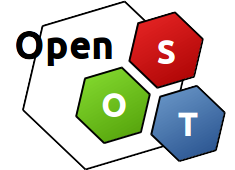
\includegraphics[width=0.25\textwidth]{images/openSoT_stickers}
  \end{center}
  \caption{OpenSoT Logo}
\end{wrapfigure}
Despite the existence of many control libraries for robotics, most of them are complex piece of software that rely on legacy code, and not easy to use for the final user. Furthermore, considering in particular the case of Inverse Kinematics (IK) frameworks, they are provided with a small set of implemented tasks and constraints. These problems make the typical IK framework a tool for just experts, ignoring the needs of a generic user who is in need of writing tasks for a complex robotic system. This work is a complement to \cite{rocchimingo:16} where the software API and tools of \textbf{OpenSoT} are presented. One of the major difference of \textbf{OpenSoT} framework with respect to other existing frameworks is the idea to \emph{collect} a comprehensive library of implemented tasks, constraints and solvers that the end-user can employ. Furthermore, the possibility to write their own tasks, constraints and solvers permits to easily enrich the existing set. This characteristic allows also to benchmark the performance of different IK problems formulations and different solvers for the same high-level tasks. 

A particular attention has been put also on the \emph{toolset} that has been developed and made available together with the library: visual markers for the Cartesian control, bindings for different programming languages, auto-generation of capsules model for the Self Collision Avoidance (SCA) constraint, a Math of Task description language and an utility library, \emph{iDynUtils} which takes care of wrapping several common robotics libraries to provide an easy-to-use comprehensive framework for robotics control (convex hull computation, self-collision checking, \emph{SE3} math). 

In this paper we also present a large set of tests and experiment to show how the framework can be used for many different high-level tasks such as walking, manipulation and interaction with the environment. We also consider different robots (simulated and real hardware) that intend to demonstrate how the library is robot agnostic.

The paper is structured as follows: in \textbf{\nameref{sec:software_architecture}} the basic API and tools are introduced, in \textbf{\nameref{sec:examples}}physical hardware and simulated  experiments are presented, and finally in \textbf{\nameref{sec:conclusions2}} some final considerations on the presented work are provided.

\subsection{OpenSoT Software Architecture}
\label{sec:software_architecture}
Designing a good Software Architecture has been a crucial step in the development of \textbf{OpenSoT}. Firstly, the design has been focused on requirements of agile programming as commanded by the tight schedules of the development for the DRC competition. The software should be straightforward to install and to use, be robust both algorithmically and at the implementation level, and allow for ease of extendability, reusability and integration with existing frameworks.

\subsubsection{Application Programming Interface (API)}
The \textbf{OpenSoT} API is structured to favor reusability.
Tasks are implemented through the class \emph{Task} which provides an interface to obtain $\A$ and $\b$, a weight matrix $W$ and a scalar weight $\lambda$ for the task (\texttt{\small getA()}, \texttt{\small getb()}, \texttt{\small getWeight()}, \texttt{\small getlambda()}).
Constraints and bounds are implemented in \textbf{OpenSoT} through the class \emph{Constraint} which implements a simple interface providing equality constraints (\texttt{\small getAeq()}, \texttt{\small getbeq()}), inequality constraints (\texttt{\small getAeineq()}, \texttt{\small getbLowerBound()}, \texttt{\small getbUpperBound()}) and bounds (\texttt{\small getLowerBound()}, \texttt{\small getUpperBound()}).

Both \emph{Task} and \emph{Constraint} classes have a pure virtual \texttt{\small update()} method to be implemented. Most of the kinematics and dynamics information are directly available inside the \emph{Task}/\emph{Constraint} thanks to a pointer to the model of the robot. The robot model (see \nameref{sec:idynutils} section) has to be updated at every control loop with measured joint position, velocities and force/torque, before the update of the IK problem as shown in Figure \ref{update}.

\begin{figure*}[!ht]
\vspace{2 mm}
\centering
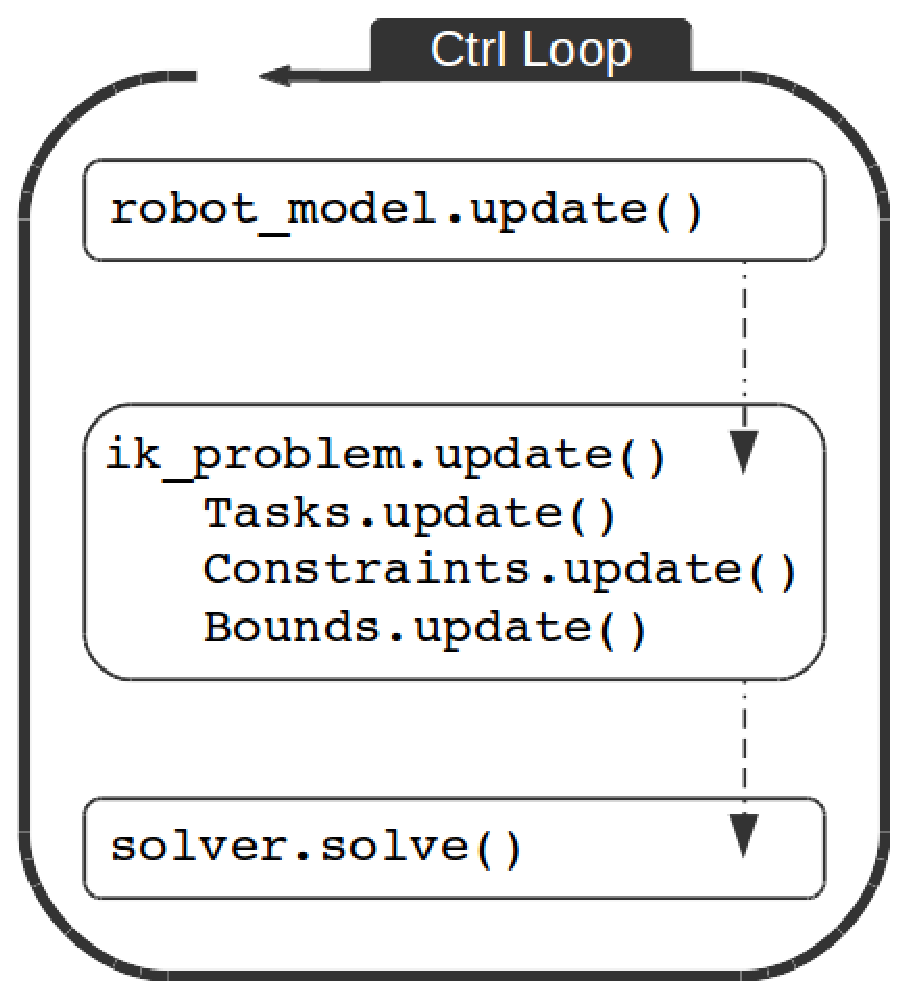
\includegraphics[width=0.25\textwidth]{images/software/update.eps}
\caption{At each control loop the robot model and the IK problem are updated and then the solver is called}
\label{update}
\end{figure*}

Controlling a new robot with \textbf{OpenSoT} requires only writing a new stack. Thanks to \nameref{sec:idynutils}, every robot which is provided with an \emph{URDF} and \emph{SRDF} can be imported for use with the library.

\textbf{OpenSoT} provide also a simple base class to write a \emph{Solver}. The main pure virtual methods consists in three constructors, depending if the solver permits to handle also bounds and constraints, and the \texttt{\small solve()} method. 

\subsubsection{Integration with Robotic Frameworks}
\label{sec:integration_with_robotic_frameworks}
By writing proper task wrappers it's possible to encapsulate the API and export the functionalities of \textbf{OpenSoT} over the network. Some wrappers are already available for the \emph{ROS} and \emph{YARP} frameworks. In particular, for \emph{ROS} the Cartesian and joint postural tasks are wrapped so that it is possible to perform simple tele-operation  through \emph{rviz}'s \emph{interactive markers}, as shown in Figure \ref{opensot_interactive_markers}.
\begin{figure*}[!ht]
\vspace{2 mm}
\centering
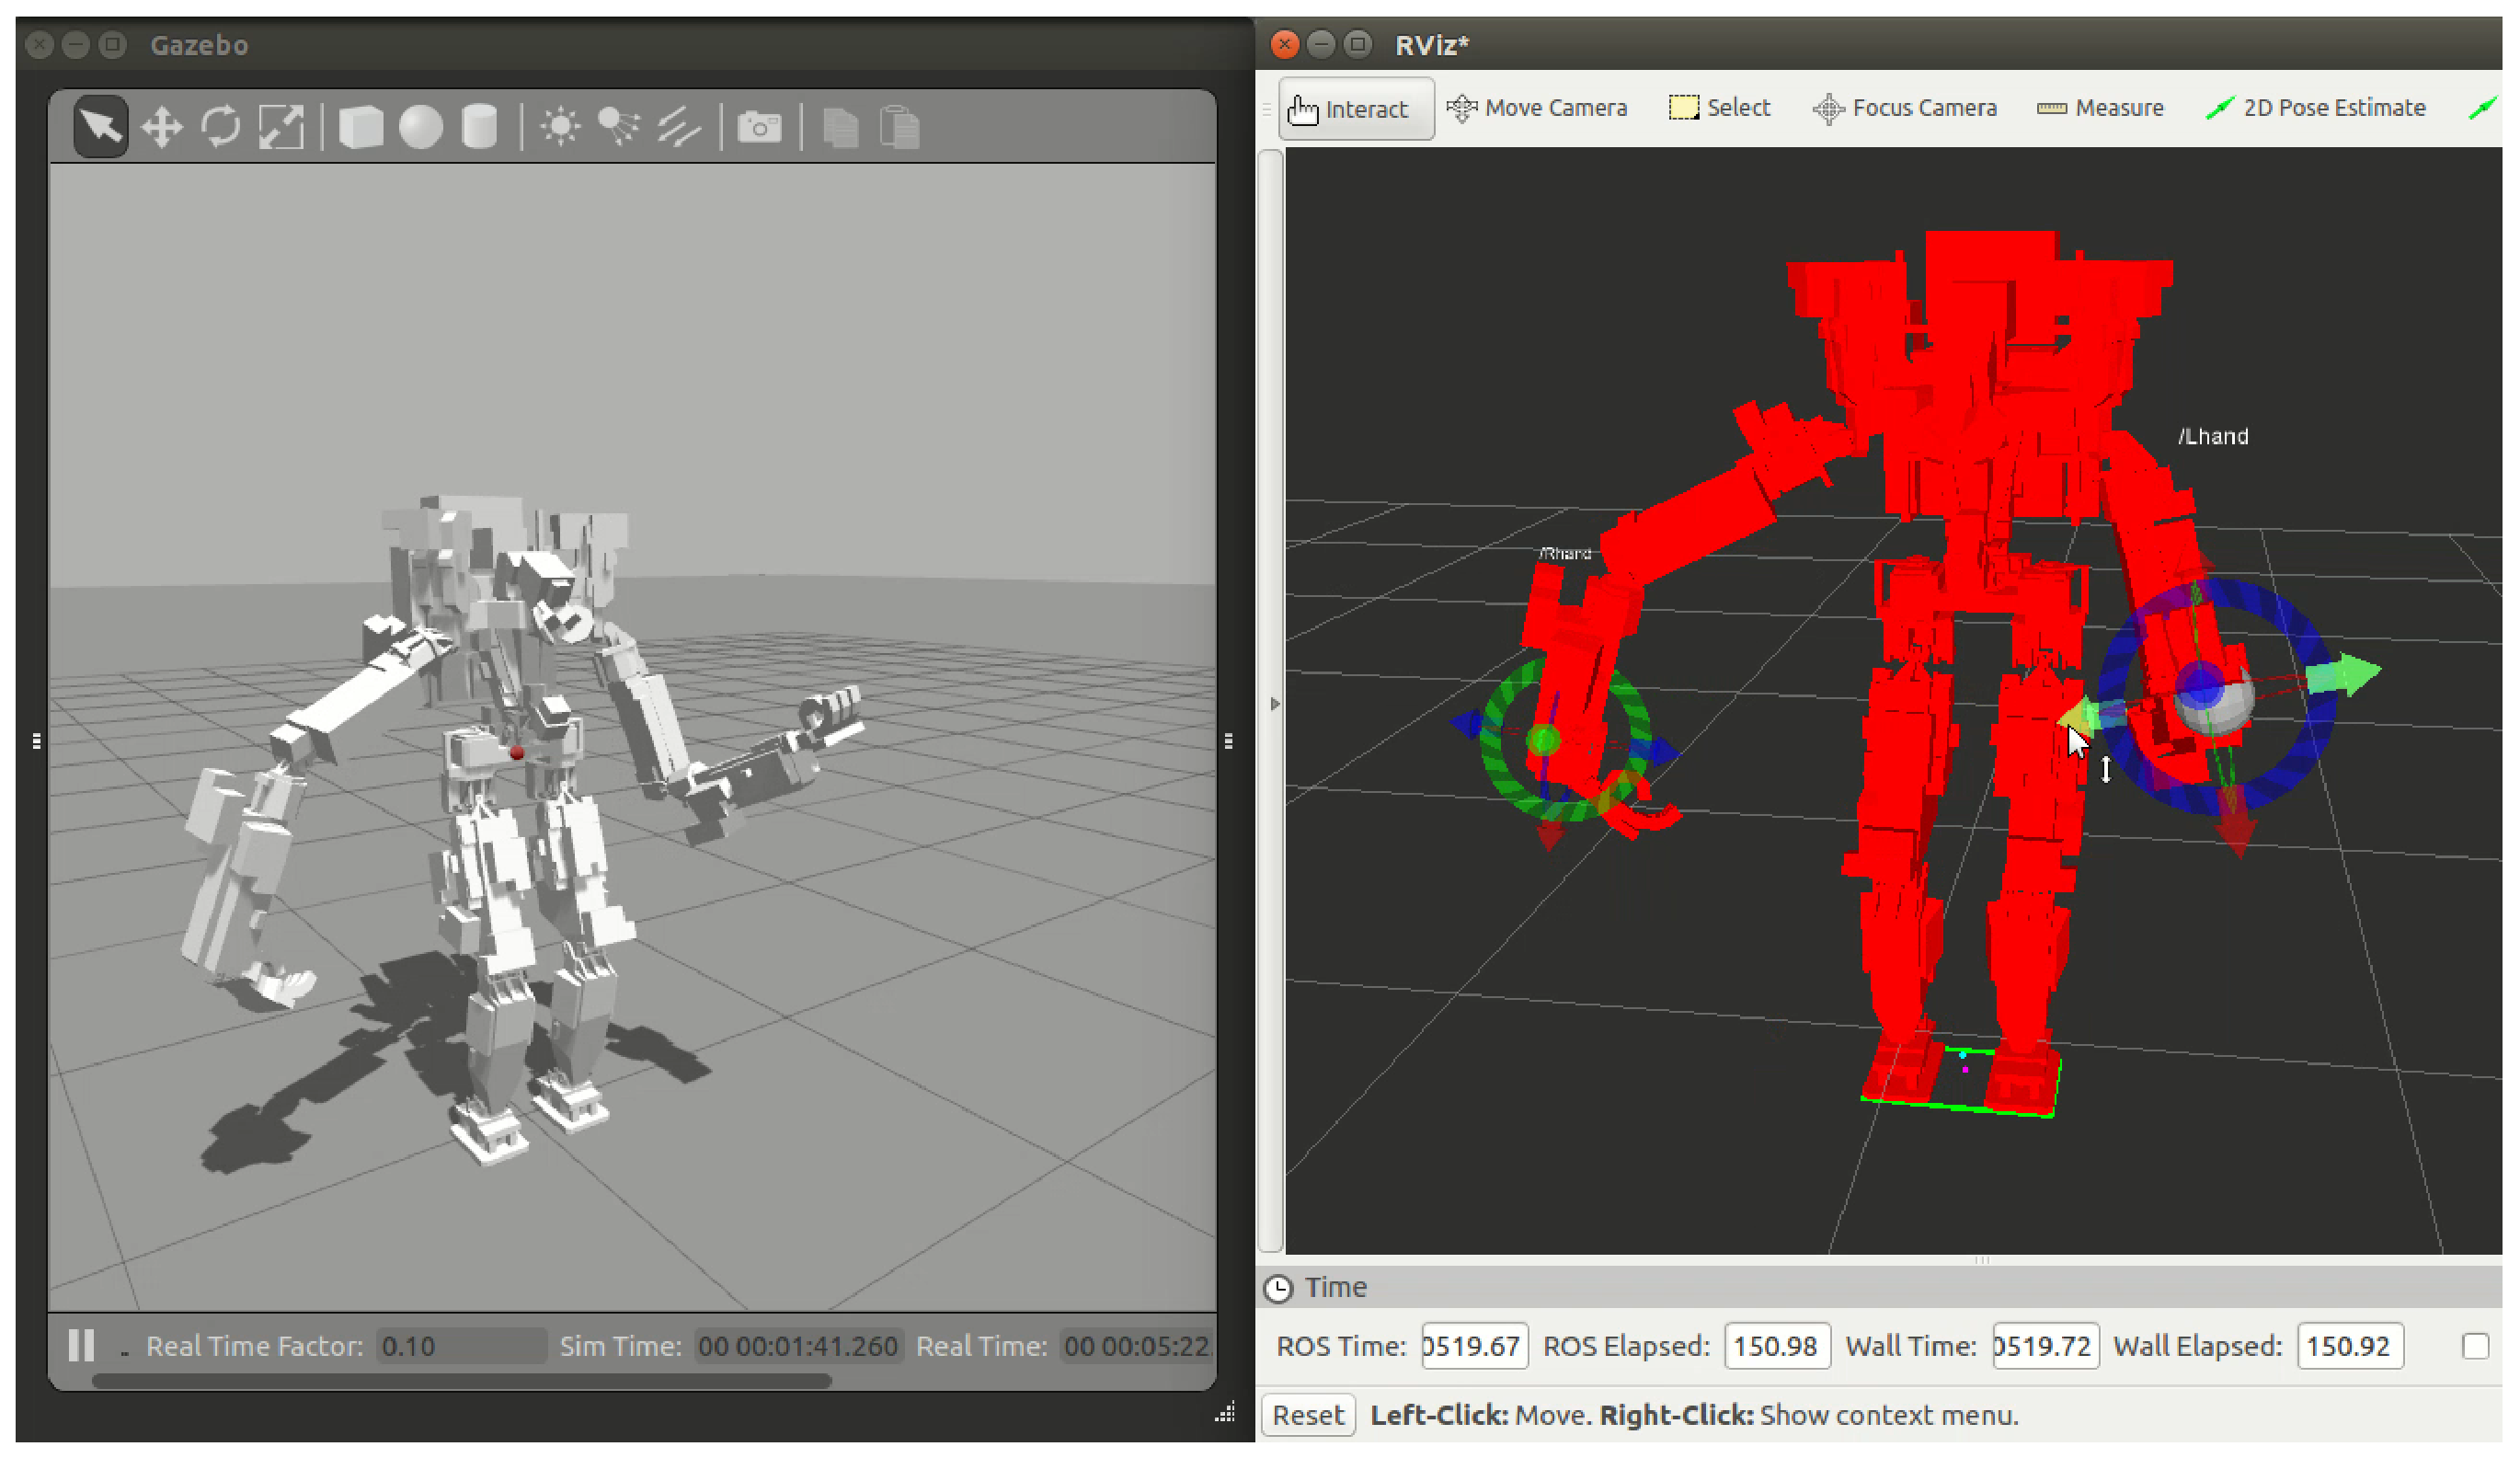
\includegraphics[width=0.7\textwidth]{images/software/hydra_tele_operation.eps}
\caption{The HYDRA robot tele-operated in simulation. The kinematic structure of HYDRA is the following: 6 DoFs legs, 8 DoFs arms, 2 DoFs torso and 1 DoF neck}
\label{opensot_interactive_markers}
\end{figure*}
Through \emph{YARP} it's possible to change the parameters of all the tasks, including $\beta$ and $\W$, and to get and set the task reference when contemplated (e.g., Cartesian, CoM, postural).

\subsubsection{iDynUtils}
\label{sec:idynutils}

As a support library to the \textbf{OpenSoT} framework we developed a whole-body control library named \emph{iDynUtils}.
This library is responsible for loading the model of the robot via the \emph{iDynTree}\cite{Nori2015-zb,Nori2015-db} library.

The library is an interface and wrapper to other robotics libraries, and provides the following functionalities:
\begin{itemize}
\item robot pose estimate w.r.t. the world via forward-kinematics based dead-reckoning
\item loop closures/kinematic constraints via kinematic tree rebasing, e.g. foot switching
\item convex hull computation via \emph{PCL}, management of link is contact with the environment with frictional constraints
\item collision and self-collision checking via \emph{Moveit!} and \emph{fcl}, helper utilities to define collision white-lists, simplified bound in volumes support (capsules management)
\item Cartesian utilities for \emph{SE3} math, in particular quaternion implementation of (17) in \cite{rocchimingo:16}%\ref{eq:cartesian_error}
\item interfaces for automatic transformation of frame of reference/poles for force/torque readings, and for frame of reference of IMU readings
\item utility functions for management of the kinematic tree as a tree or as as a list of chains
\end{itemize}
In particular with respect to item 1, 2 and 3, the structure of the library makes so that the dead-reckoning is a simple integrator based on the forward kinematics of the robot.
In particular, among the links in contact with the environment, we select a link which will be called the  \emph{anchor} for the dead-reckoning phase, and a link to which the \emph{floating base} will be attached. While the computation of the IK problem's solution can take into account explicitly the virtual joints of the floating base, most of the tasks already implemented in \textbf{OpenSoT} will follow an approach where the Jacobians are cut to take into account only the actuated joints. In this way, the solution of the problem will be computationally less intensive as the Hessian of the equivalent QP problem will be smaller, and we will drop the chain-closure constraint (i.e., imposing that the chain going from the \emph{anchor} link to the world through the floating base virtual chain will have only internal movements, or alternatively, the twist of the \emph{anchor} link with respect to the world frame will be $0$). For this reason, the \emph{iDynUtils} library has been implemented to provide functionalities for both use cases, and in particular the \emph{anchor} and \emph{floating base} links can be coincident, and during a typical walking phase, they will switch from one support foot to the other (with the switch command given by the walking algorithm), and remain constant during the double support phase.

\subsubsection{Python Bindings}
A set of bindings is provided for the \textbf{OpenSoT} framework that allow to send commands to an existing stack that runs as a server. While the stack needs to be defined and compiled in C++ at the moment, the approach allows to program the tasks in python using simple interfaces. In particular, python interfaces are available to allow the creator of python clients for the \emph{YARP} bindings (introduced in \ref{sec:integration_with_robotic_frameworks}) to \textbf{OpenSoT}. The python bindings ease the process of creating messages for the \emph{YARP} interfaces, namely \texttt{pose} messages, \texttt{twist} messages, \texttt{joint position} messages and \texttt{trajectory} messages. Using these, the \texttt{YTask} python binding defines a generic binding to a task with a \emph{YARP} interface (a \emph{YTask}), such as getting and setting weights and gains. The \texttt{CartesianTask}, \texttt{CoMTask} and \texttt{PosturalTask} extend the base class \texttt{YTask} to provide specific functions to set and get references for the corresponding \emph{YARP} interfaces to the corresponding tasks, as written in C++ (see Figure \ref{fig:python_binding} for details).
An example is provided to generate generic bindings via \emph{SWIG} for interfacing with the \emph{Klampt} simulator.
\begin{figure*}
\vspace{2 mm}
\centering \includegraphics[width=0.6\textwidth]{images/software/python_markers.eps} 
\caption{Integration of Python and RVIZ markers inside \textbf{OpenSoT}} 
\label{fig:python_binding}
\end{figure*}


\subsubsection{Integration with Generic Simulators}
While \textbf{OpenSoT} has been used extensively with Gazebo, using an abstraction infrastructure that allowed to seamlessly switch from the physical robot to the simulated robot \cite{hoffman2014yarp}, the \textbf{OpenSoT} library is generic and can be used with any simulation and control infrastructure.
A suggested workflow for using \textbf{OpenSoT} with simulators and controllers written in C++ and python is provided in the examples. While the library \nameref{sec:idynutils} is model-based, and the model is populated using URDF and SRDF descriptions of a robot, the main steps for connecting the library to a generic software is to specify conversion functions to transform joint positions and references between the simulator and the \textbf{OpenSoT}-based controller.
The suggested way consists in transforming the joint reading vectors specified by the simulator in a joint readings map that associates the joint names with joint values, in a similar way to what \emph{ROS} enforces via joint state messages and \emph{YARP} implicitly does in the \emph{Gazebo YARP plugins}. The same is done in \textbf{OpenSoT} to transform the joint readings map into its joint readings vector (in general the two vectors might assume different joint indices). Once specified this lightweight translation layer that uses sensors names to exchange data, \textbf{OpenSoT} can be encapsulated in the custom simulation/controller architecture. An example of a \emph{HUBO} robot being simulated in the \emph{Klampt} simulator is shown in Figure \ref{fig:HUBO}, where the stack for the three tasks is a whole body stack composed of
\begin{equation}
\begin{pmatrix}

\left(T_{\substack{\text{Right}\\\text{Foot}}} + T_{\substack{\text{Left}\\\text{Foot}}}\right)\setminus\\
\\
T_{\text{CoM}_\text{XY}}\setminus\\
\\
T_{\text{Waist}_\text{Z}}\setminus\\
\\
\left(T_{\substack{\text{Right}\\\text{Wrist}}} + T_{\substack{\text{Left}\\\text{Wrist}}}\right)\setminus\\
\\
T_{\substack{\text{Joint}\\\text{Postural}}}

\end{pmatrix}
<< \left(B_{\substack{\text{Joint}\\\text{Limits}}} + B_{\substack{\text{Joint Velocity}\\\text{Limits}}}\right)
\end{equation}
and velocity allocation strategy (see \nameref{velocity_allocation}).
The Hubo robot used in the simulation has a $1$ DoFs torso, $6$ DoFs legs and arms, $2$ DoFs neck, $15$ DoFs arms. Figures \ref{fig:HUBO} are generated by using \emph{Gazebo}. Notice how the two simulators use a different approach to controller simulation, whereas in \emph{Klampt} we have a synchronous execution of the controller together with the simulator, while in \emph{Gazebo} the controller runs asynchronously and needs to be synchronized by using the simulation clock, so as to obtain a simulated real-time execution on the controller.

\subsubsection{Notes on Robustness}
The \textbf{OpenSoT} framework has been developed with stability and robustness in mind, both at the algorithmic level, and at the software level. Best practices for software development are crucial when working in big groups of people under a tight deadline. For this reason, a set of unit and integration tests has been developed, which where possible also generate simulation data and graphs for human inspection. On the debugging side, the solver dumps the QP problem stack once a failure in solving the a problem is encountered, which allows for inspection and reproduction.

\subsubsection{Utilities}
Other than the \nameref{sec:idynutils} package, several utilities have been developed as \textbf{OpenSoT} ancillaries. Between these, the \nameref{subsub:CapsuleGeneration} toolkit and the \nameref{subsec:Previewer} class. The former allows to generate simplified bounding volumes for the robot links' geometries, as required by the collision avoidance task as defined in section Self-Collision Avoidance Constraint in \cite{rocchimingo:16}. %\ref{sec:collision_avoidance}.
The latter allows to automatically check for a defined motion before executing it on the robot, by kinematically simulating a certain task while checking user-defined convergence and maximum error thresholds, and checking for self-collision. In particular, the \nameref{subsec:Previewer} is implemented to so be used programatically to generate a Task workspace for a given stack and robot.

\paragraph{Capsule Generation}
\label{subsub:CapsuleGeneration}
In order to compute the minimum distance between links, an automated way to generate capsule approximation of meshes for URDF model is needed. To this extent, we developed tools using the \emph{Roboptim} \cite{Moulard2013-nk,Moulard_undated-tm} numerical optimization for robotics library. Through the plugin \emph{roboptim-capsule} the library finds the minimum volume capsule that contains the given polyhedra. The optimization problem resolving in optimal capsules is reported here for convenience \cite{el_khoury2013-rp}

\begin{eqnarray*}
\min_{e1,e2,r} & \left\Vert e_2 - e_1 \right\Vert_2 \pi r^2+\frac{4}{3}\pi r^3\\
{s.t.}  & r-d(p,e_1e_2) \ge 0, & \vee p \in P
\end{eqnarray*}

where $p$ is a vertex of the polyhedron $P$ and we want to find the capsule of minimum volume for which the distance $(p,e_1e_2)$ between $p$ and the segment $e_1e_2$ is smaller than the capsule radius.

The integration of the plugin with our architecture needs to circumvent the lacking of the capsule primitive in the URDF format and on all the ecosystem of libraries using the URDF format, including the popular interface \emph{rviz}.
Once our wrapper analyzes the URDF file of the model described with meshes, it will convert them to the corresponding capsules via the \emph{roboptim-capsule} optimization, and create an URDF file with cylinders in place of meshes. The wrapper takes care to transform the capsule parameters between the endpoints-radius representation and radius,length,center representation during the process, in order to integrate the different components of the system.
The self collision avoidance constraint then will scan the URDF looking for cylinders and interpret them as the body of a capsule, to feed the \emph{fcl} library which takes care of computing minimum distances between the robot links using the simplified bounding volume. 
An example of application of this method on different robotic platforms can be seen in Figure \ref{fig:capsules}.
\begin{figure*}
\vspace{2 mm}
\centering 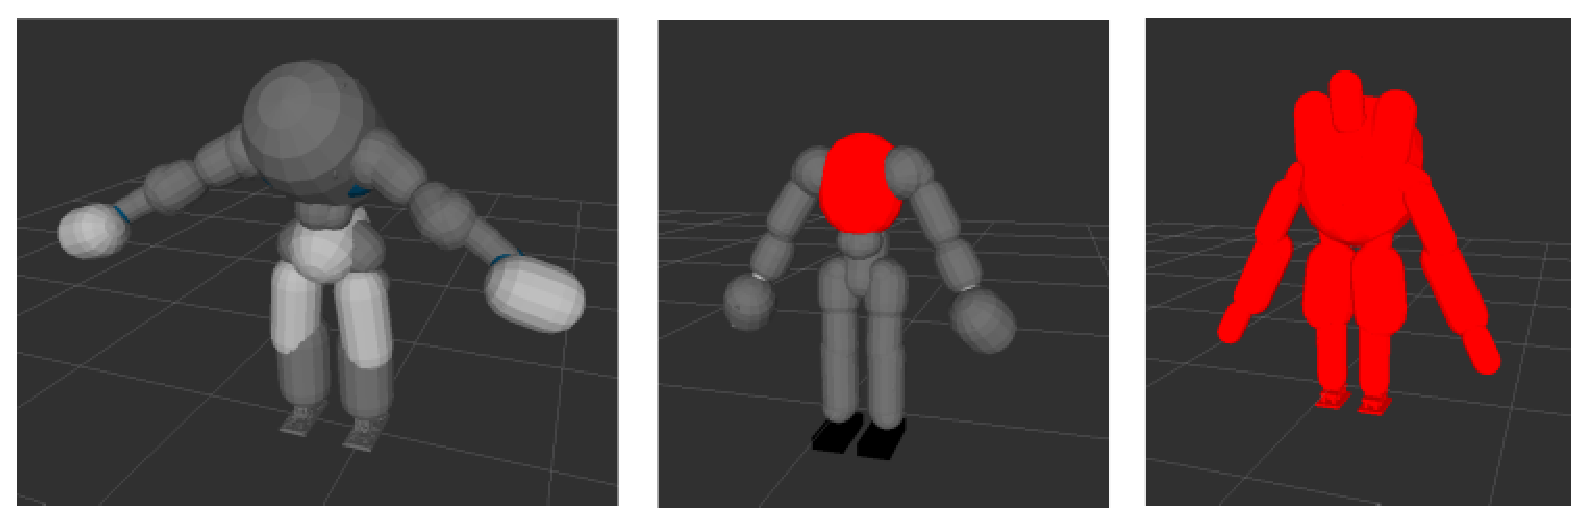
\includegraphics[width=0.8\textwidth]{images/software/robots_capsules.eps} 
\caption{Generated capsule models for WALK-MAN, COMAN and HYDRA respectively} 
\label{fig:capsules}
\end{figure*}
One last step after the generation of the capsule lies in creating the collision whitelists, that is, the default pairs of links to check for collision detection in the robot. This process is performed by the \emph{moveit setup assistant}\cite{Coleman2014-bd} library, which randomly samples the joint configuration space, applies FK for each sample and finds link pairs which are always in collision and link pairs which are never in collision. These lists are then stored into the SRDF file for later use by the self-collision avoidance algorithm: the link pairs which do not fall in this category are in fact put in the white-list for collision detection.

\paragraph{Previewer}
\label{subsec:Previewer}
An architecture for previewing actions kinematically in Operational space before executing them on the robot (or in a dynamic simulation) is provided in order to automatically check for the feasibility of a certain movement. The interface of the previewer \emph{previewer} to \emph{bind} a trajectory generator to a \emph{Task}. During the execution of the task trajectory, the \emph{previewer} will check several parameters to ensure that the task can be executed (Figure \ref{fig:previewer}). In case the joint-space configuration diverges significantly from the previous one, it will perform a self-collision check. All these parameters can be tuned, and are exemplified in Table \ref{table:previewer_constants}.

The \emph{Previewer} will return with a results log containing error events, and can be configured with a callback, which can be used for example to publish the joint status of the robot while performing the action preview to \emph{ROS}.
The error log for the \emph{Previewer} will contain events in the class
\begin{itemize}
\item collision
\item Cartesian error unbounded
\end{itemize}
while the results log will keep track of the trajectory $(t,\q)$ and of the Cartesian errors associated to the task execution along the trajectory, namely the moving average of the error norm, the current error norm, and the current Cartesian error, together with the Cartesian error to the goal, where the Cartesian error is defined as in (17) in \cite{rocchimingo:16}
\begin{figure*}
\vspace{2 mm}
\centering 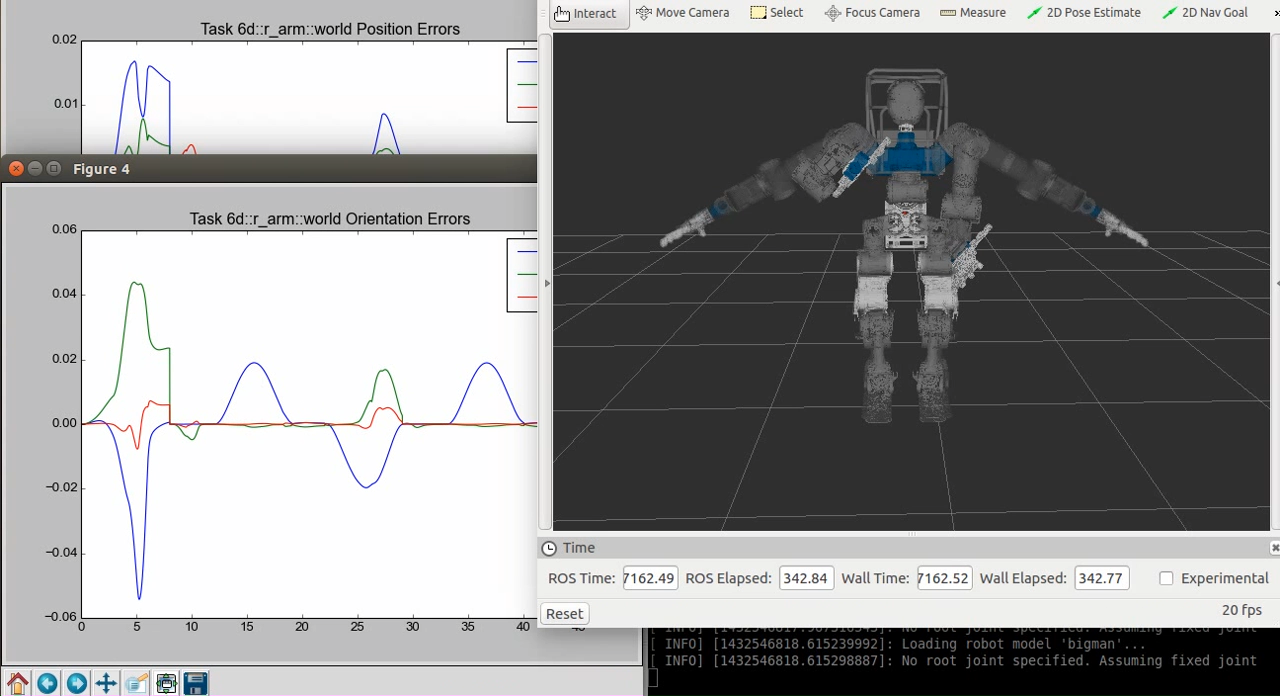
\includegraphics[width=0.7\textwidth]{images/software/previewer} 
\caption{The phantom model is superposed to the robot model to show the motion that the robot will perform. Plot of the trajectories are automatically generated by the previewer} 
\label{fig:previewer}
\end{figure*}

The success of the action will be determined according to the settings of the previewer, and the specified duration of the preview action. In fact, a user can decide to preview an action partially, and get results from that partial preview of an entire trajectory, or preview an action till convergence is detected. The success is determined when no error conditions where raised during preview, and one of the following convergence conditions is true at the end of the preview action:
\begin{itemize}
\item Cartesian error is small
\item Cartesian error is small and not decreasing
\item Cartesian error is small, not decreasing, and joint velocities are below a user-defined threshold (null-space tasks converged) 
\end{itemize}

\begin{table}[hbt]
   \small
   \begin{center}
   \begin{tabular}{| >{\centering\arraybackslash}m{2.3in} | >{\centering\arraybackslash}m{0.5in} | >{\centering\arraybackslash}m{3in} |}
   \hline
   \textbf{Constant} & \textbf{Default Value} & \textbf{Meaning} \\\hline
   \cline{1-3}
   \texttt{TRAJECTORIES\_EXPIRED\_SAFETY\_MARGIN}           & $1.5$   & \shortstack{when previewing for an infinite time, stop \\ \texttt{if t >= longest\_task\_duration * safety\_margin}} \\\hline
   \texttt{UPDATE\_ERR\_STATS\_WINDOW\_SIZE\_IN\_SECS} & $0.1$    & \shortstack{set the time window of the moving average filter \\ for the error statistics} \\\hline
   \texttt{PREVIEWER\_CHECK\_MAX\_RETRIES}                  & $3$     & if \texttt{solve()} fails, retry for a maximum of MAX\_RETRIES \\\hline
   \texttt{TRAJ\_BINDING\_MAXIMUM\_ALLOWED\_ERR}           & $5\times10^{-2}$  & \shortstack{maximum allowed Cartesian error, in norm, \\ during task execution} \\\hline
   \texttt{TRAJ\_BINDING\_CONVERGENCE\_TOLERANCE}           & $5\times10^{-4}$  & threshold value for Cartesian error norm convergence \\\hline
   \end{tabular}
   \end{center}
   \caption{Constraints and bounds. Transforming unilateral constraints and bounds from upper bounds to lower bounds is trivial and therefore not included in the table}
   \label{table:previewer_constants}
\end{table}

\section{Conclusions}
While in previous section the theoretical foundations of the high level control framework we addressed, together with a large set of experiments, in this section the API, the software infrastructure and the utilities ecosystem has been addressed, with the intent of demonstrating the richness of features of our high level control scheme.
Statistics and best-practices used in the WALKMAN team have been presented as part of the work for the DRC competition. Lastly, the simulation, middleware and component model used by the team has been presented as a fundamental scaffolding of the work of the team and as a means of organizing the work of the team.